\chapter{Signs}
	\section{Introduction}
	\paragraph{}Signs main objective is to give some information to the pilots about what lies ahead in order to guarantee the perfect organisation and efficiency of the aircraft trajectory while on taxiways. 
	
	The criteria used in order to dimension and calculate the position of each sign can be obtained from a table stated on the point 5.4 of the Annex 14.
	
	\begin{figure}[H]
		\centering
		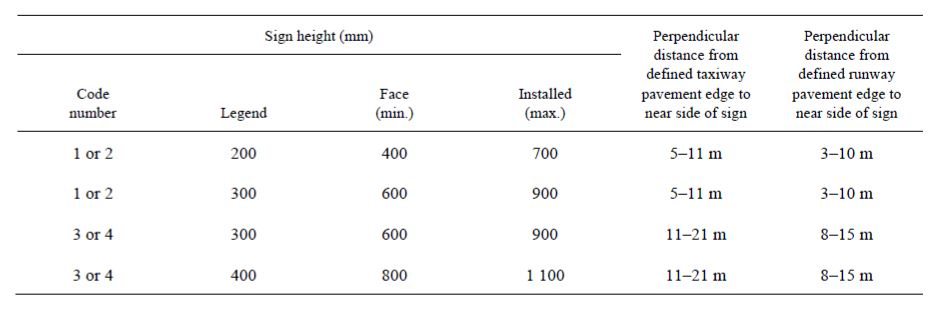
\includegraphics[clip, trim=0cm 0cm 0cm 0cm, width=0.95\textwidth]{./images/Annex14/signstable}
		\caption{Location distances for taxiing guidance signs.} %nom de la figura
		\label{} %per denotar una referencia
	\end{figure}

	Since the airport designed has a number reference of 4, the distance from the runway to the sign will be 12m and the distance from the taxiways will be 15m. Two different values have been chosen in order to help the pilots differentiate which sign are they looking at. 
	
	Another important aspect to be taken into account is the fact that all the signs will have inside illumination in order to allow the night time operations.
	
	\section{Mandatory instruction signs}
	\textbf{\textit{Application}}
	
	A mandatory instruction sign shall be provided to identify a location beyond which an aircraft taxiing or vehicle shall not proceed unless authorized by the aerodrome control tower. The signs included in this section are: designation signs, category I, II or III holding position signs, runway-holding position signs, road-holding position signs and NO ENTRY signs.
	
	\textbf{\textit{Location}}
	
	The location of each sign depend on the prohibition or the information they are giving:
	
	- A runway designation sign at a taxiway/runway intersection or a runway/runway intersection shall be located on each side of the runway-holding position marking facing the direction of approach to the runway.
	
	- A category I, II or III holding position sign shall be located on each side of the runway-holding position marking facing the direction of the approach to the critical area.
	
	- A NO ENTRY sign shall be located at the beginning of the area to which entrance is prohibited on each side of the taxiway as viewed by the pilot.
	
	\textbf{\textit{Characteristics}}
	
	A mandatory instruction sign shall consist of an inscription in white on a red background. Furthermore, in the specific case of inscription on a category I, II, III, joint II/III or joint I/II/III holding position sign shall consist of the runway designator, it must be followed by CAT I, CAT II, CAT III, CAT II/III or CAT I/II/III, as appropriate.
	
	\section{Information signs}
	\textbf{\textit{Application}}
	
	An information sign shall be provided where there is an operational need to identify by a sign, a specific location, or routing information. Furthermore, information signs shall include: direction signs, location signs, destination signs, runway exit signs, runway vacated signs and intersection take-off signs.
	
	\textbf{\textit{Location}}
	
	Wherever practicable, the signs must be located on the left-hand side of the taxiway in accordance with table shown at the beginning of the section. Depending on the information sign, they get a different location:
	
	-At a taxiway intersection, information signs shall be located prior to the intersection and in line with the intermediate holding position marking. Where there is no intermediate holding position marking, the signs shall be installed at least 60 m from the centre line of the intersecting taxiway where the code number is 3 or 4, and at least 40 m where the code number is 1 or 2.
	
	- A runway exit sign shall be located prior to the runway exit point in line with a position at least 60 m prior to the point of tangency where the code number is 3 or 4, and at least 30 m where the code number is 1 or 2.
	
	\textbf{\textit{Characteristics}}
	
	A location sign shall consist of an inscription in yellow on a black background and where it is a stand-alone sign shall have a yellow border and the inscription on a runway exit sign shall consist of the designator of the exit taxiway and an arrow indicating the direction to follow.
	
	